\subsection{Subsample}
\label{subsection:subsample}

\begin{figure}[!h]
\begin{center}
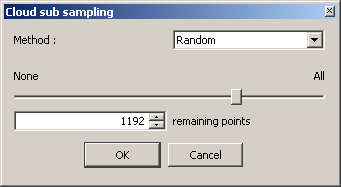
\includegraphics[width=0.4\textwidth]{Partie3_Fonctions/subsamplingDlg.png}
\caption{\label{fig:subsamplingDlg}Interface de param�trage pour le sous-�chantillonnage de nuages}
\end{center}
\end{figure}

\index{echantillonner@�chantillonner!sous-echantillonner@sous-�chantillonner}
Fonction de sous-�chantillonnage des points d'un nuage.\\
\par
Diff�rentes m�thodes sont disponibles. Le choix (ainsi que le param�trage) se fait via une bo�te de dialogue (voir figure~\ref{fig:subsamplingDlg}) :
\begin{itemize}
\item \emph{Random} : sous-�chantillonnage al�atoire (les points sont tir�s au hasard). L'utilisateur choisit le nombre de points restants.
\item \emph{Space} : sous-�chantillonnage spatial. L'utilisateur choisit la densit� du nuage r�sultant via l'espace moyen inter-points maximal (valeur approximative).
\item \emph{Octree} : sous-�chantillonnage rapide via l'octree\index{octree}. On garde un point par cellule de
l'octree � un niveau donn� de subdivision. L'utilisateur choisit le niveau de subdivision (plus le niveau est faible et moins le nombre de points est important).\\
\end{itemize}
\par
Remarques :
\begin{itemize}
\item Le \textbf{sous}-�chantillonnage diff�re du \textbf{r�}-�chantillonnage (cf. section~\ref{subsection:resampleWithOctree}) dans le sens o� il ne cr�e pas de nouveaux points mais se contente de s�lectionner un sous-ensemble de points � partir du nuage source.
\item La m�thode de sous-�chantillonnage rapide via l'octree choisit le point le plus proche du centre dans chaque cellule. Ainsi l'�cart entre les points est � peu pr�s constant (si le nuage initial est suffisamment dense).
\end{itemize}
